An image is generated where only the pixels at the border or the lesion are visible, the rest of the image is black. The pixels are gathered sequentially into an array starting at any arbitrary border pixel and traversing the border continually. It's important that the sequential order of the pixels be maintained since the change in angle and distance to the lesions center will be measured.

\begin{figure}[H]
    \centering
    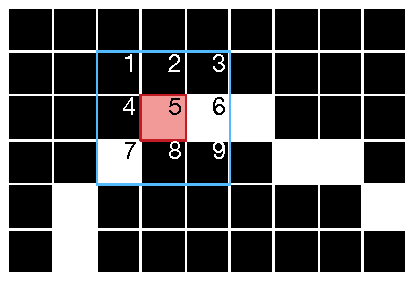
\includegraphics[height=7cm,keepaspectratio]{assets/border/travers_grid.pdf}
    \caption{Traverse the border sequentially}
    \label{fig:tra_border}
\end{figure}

An algorithm was developed that finds an arbitrary border pixel in an image that is otherwise black by iterating though pixels starting at the top left corner. When it has found a pixel that is not black it tests neighboring pixels, starting with the upper left neighbor and traversing the pixels row by row starting from the left most pixel in a row, as illustrated by the numbered pixels in figure \ref{fig:tra_border}. The center pixel, pixel number 5, is skipped.

When a non black pixel is detected it is compared to a a list or previously detected pixels. If it has not been previously detected, it is added to the list and becomes the new center. The algorithm is repeated.

If no new non-black pixel is detected the outter range is expanded by one pixel at each edge and the pixels at the edge of a 5 x 5 area are tested. This is repeated until a new pixel is found. This prevents the algorithm from halting if there are discontinuities in the border.

When the algorithm reaches the starting pixels it ends. The list of pixels now contains a sequential list of pixels that are in sequential order.

For each pixel the distance and angle from the lesion's center of mass is calculated. If a lesion's border is irregular the measure of distance and angle from the center will be erratic, whereas is the border is relatively circular and smooth the measure of distance and the difference in angle will not change abruptly between neighboring pixels.

The distance function is averaged around the distance of the start pixel (set to zero) in order to reduce discontinueities. A gaussian lowpass filter is used to reduce noise and aliasing artifacts due to pixelization.

From the smoothed distance function the first derivative is calucalated. From the angle function the difference from neighboring pixels is calculated. The resulting two functions are split into 8 equal segments. Each segment is analysed for strong variations in distance and sign changes in the difference of the angles. A sign change would indicate a very strong change in direction of the border function. For each segment in which strong variations are detected a point in the B score is added.

A lesion with strong variations in one segment, but otherwise smooth border function would have a B score of 1, whereas a lesion with variation is each of the 8 segments would have a B score of 8.

\begin{figure}[H]
    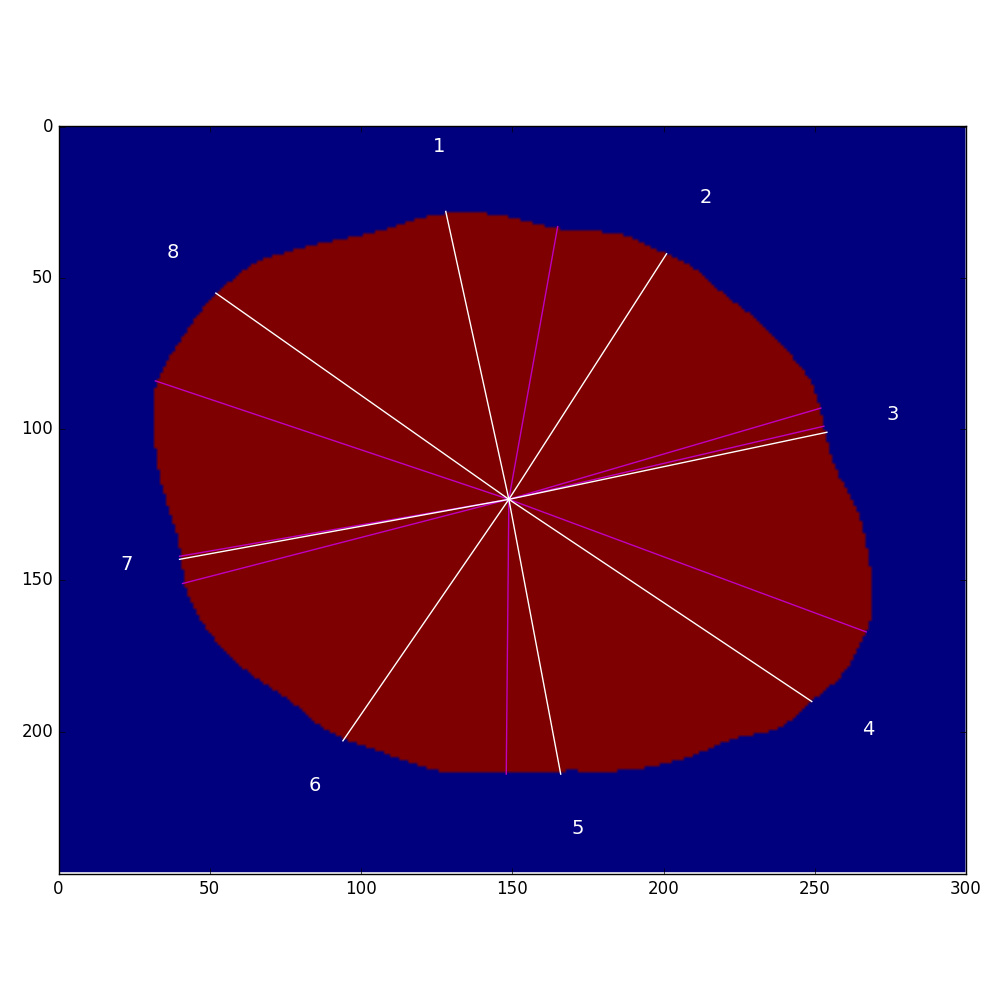
\includegraphics[height=7cm,keepaspectratio]{assets/border/examples/border_0/border.png}
    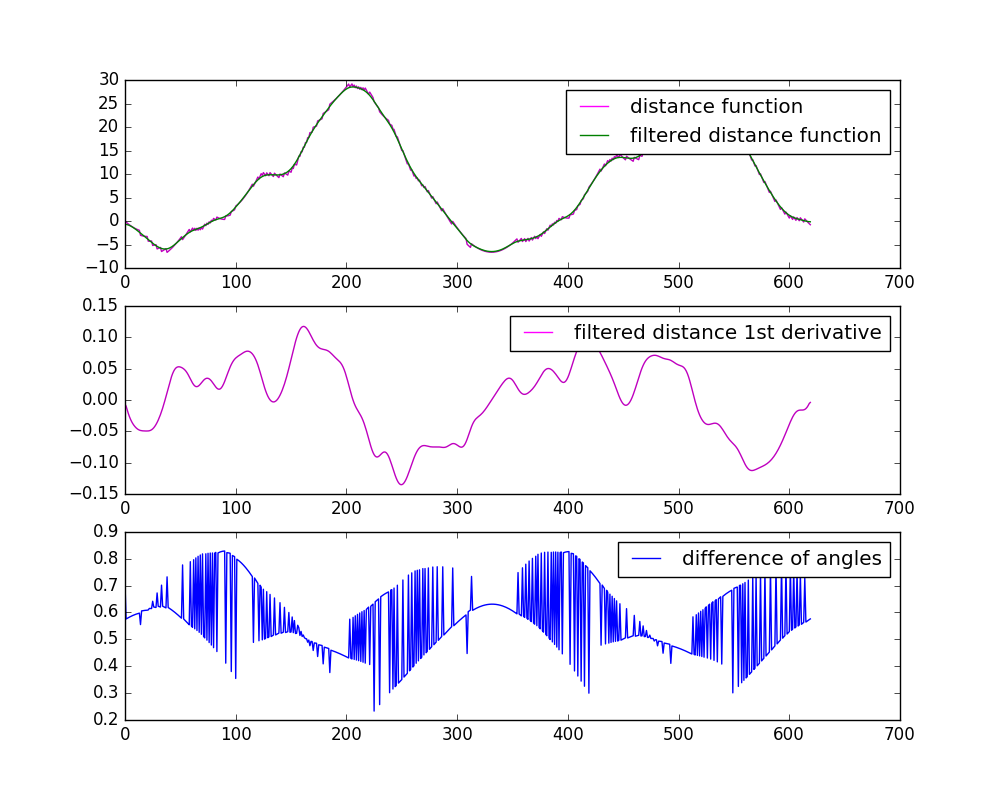
\includegraphics[height=6cm,keepaspectratio]{assets/border/examples/border_0/figure_1.png}
    \caption{Example of border score 0}
    \label{fig:border_0}
\end{figure}
\begin{figure}[H]
    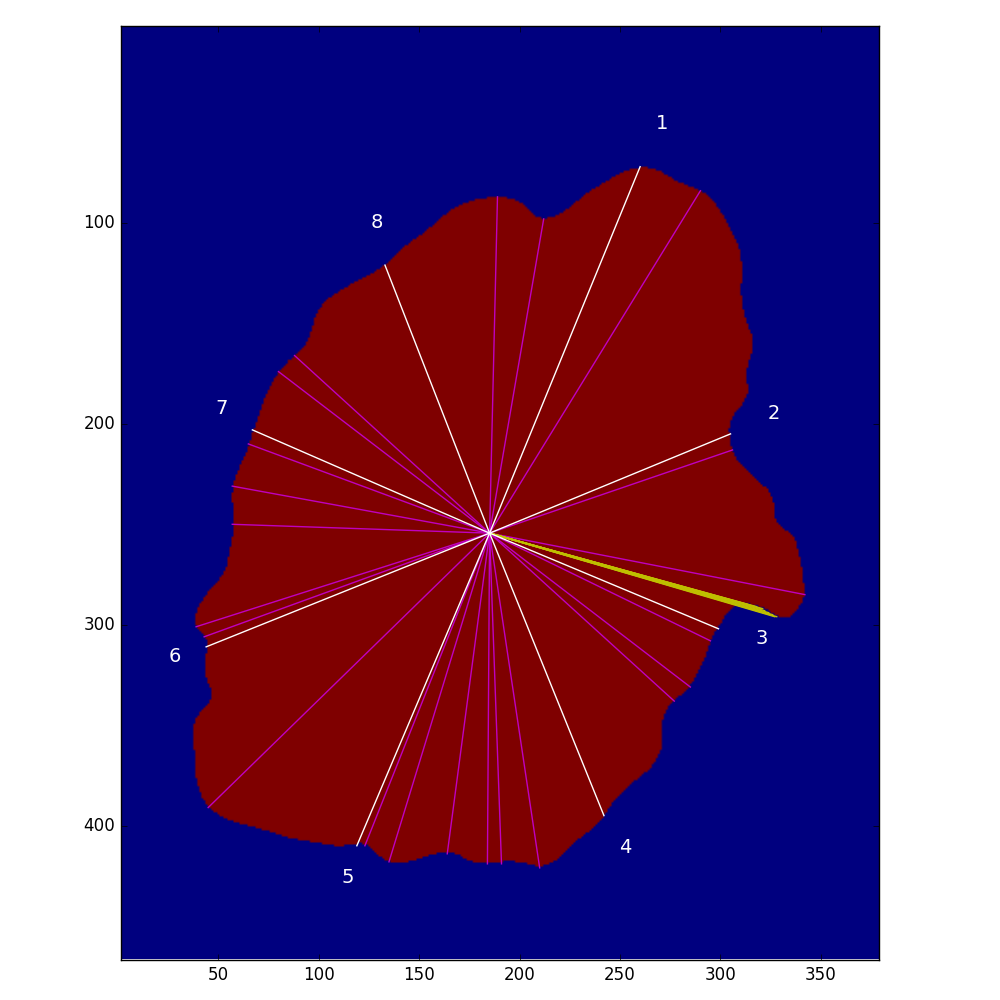
\includegraphics[height=7cm,keepaspectratio]{assets/border/examples/border_4/border.png}
    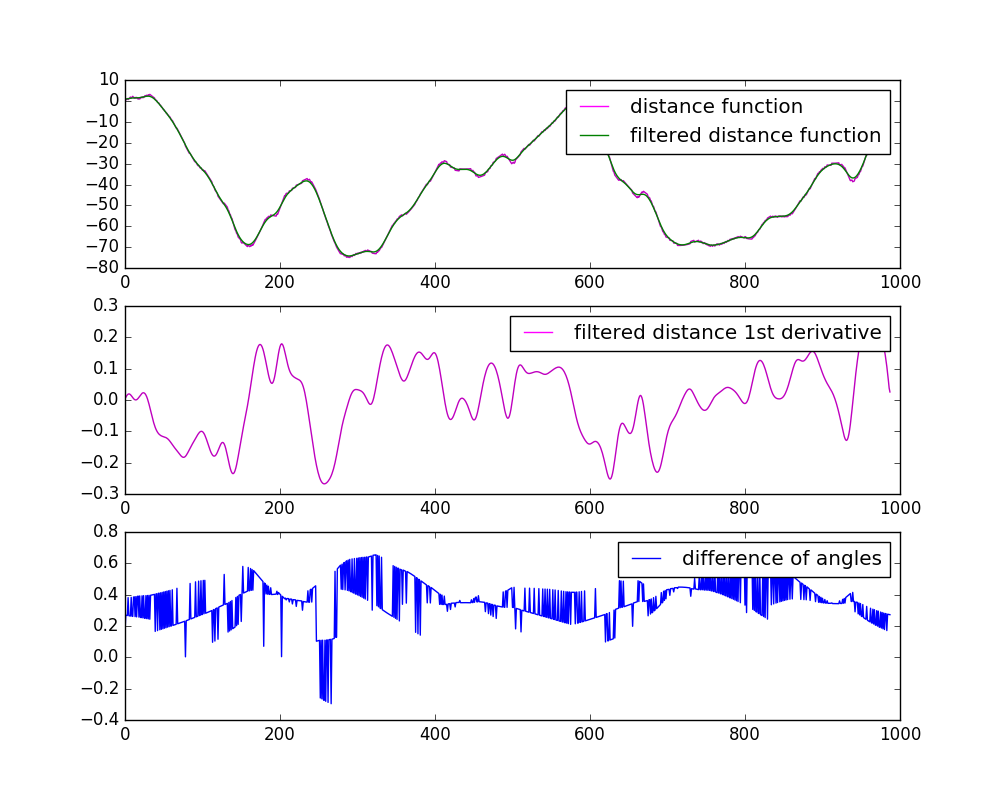
\includegraphics[height=7cm,keepaspectratio]{assets/border/examples/border_4/figure_1.png}
    \caption{Example of border score 4}
    \label{fig:border_4}
\end{figure}
\begin{figure}[H]
    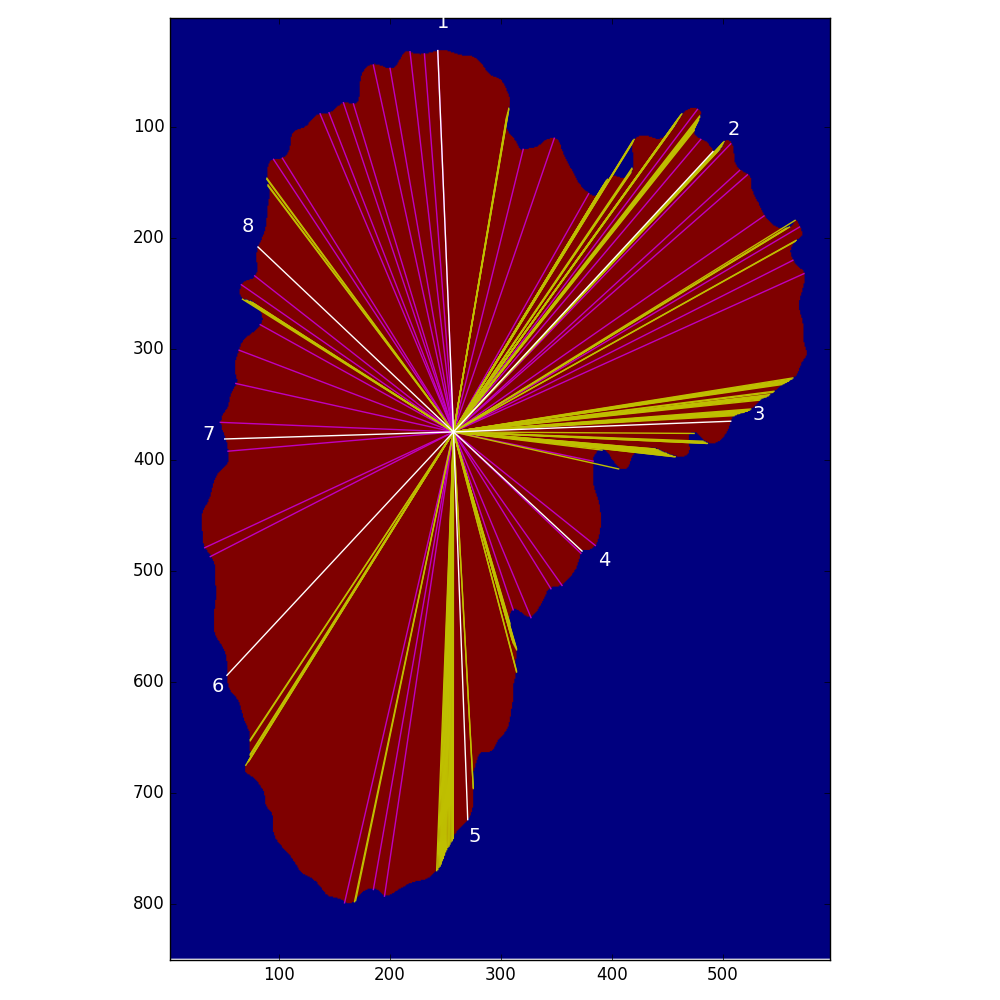
\includegraphics[height=7cm,keepaspectratio]{assets/border/examples/border_8/border.png}
    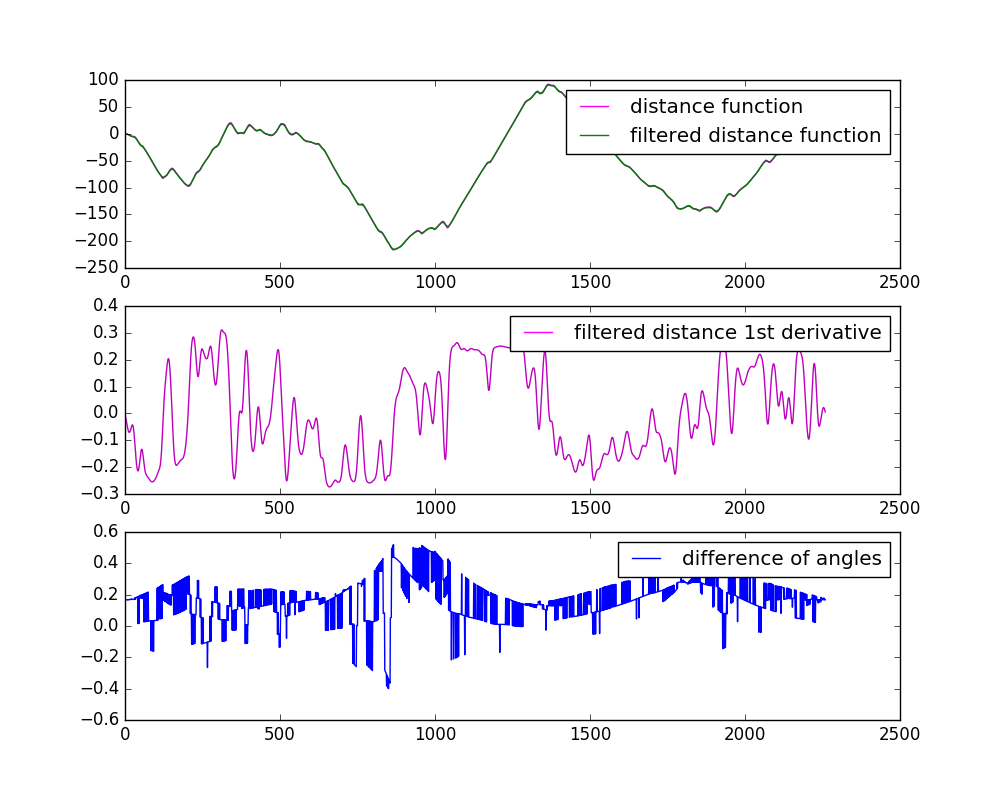
\includegraphics[height=7cm,keepaspectratio]{assets/border/examples/border_8/figure_1.png}
    \caption{Example of border score 8}
    \label{fig:border_8}
\end{figure}


